\chapter{Theoretical background}
This chapter outlines the principles and components of indoor positioning systems, including common measurement and positioning methods. Here, we discuss the technical foundations of wireless technologies used in IPS, focusing on UWB and describing its signal structure, modulation schemes, and ranging mechanisms. The chapter also identifies key error sources in UWB systems, such as NLoS propagation, setting the stage for the mitigation strategies proposed in the following chapter.

\section{IPS overview}
Indoor positioning systems are used to determine the location of the target within the indoor space. The majority of the IPSs use wireless technologies, including BLE, Wi-Fi, and UWB~\cite{singh2024systematic}.

\begin{figure}[tbh]
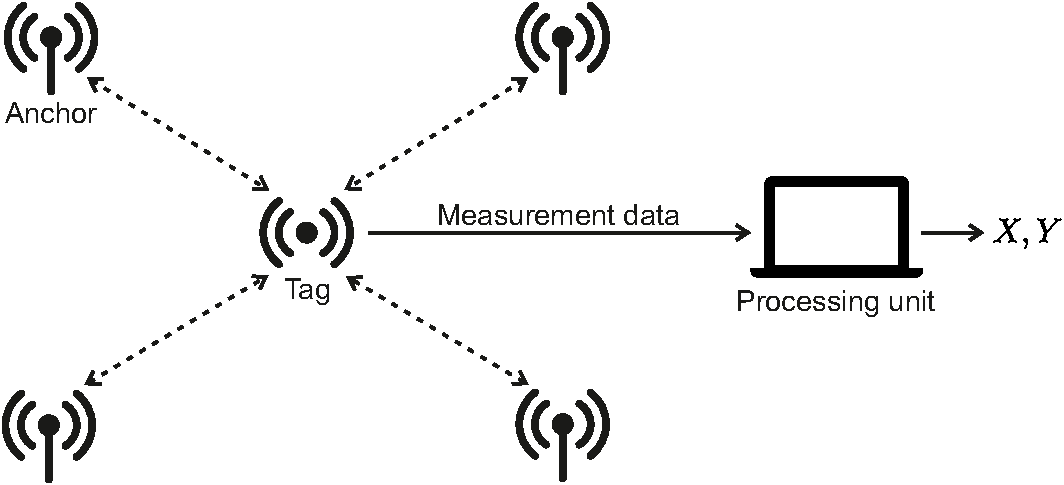
\includegraphics[width=0.75\textwidth]{Figures/theoretical_background/ips_topology.pdf}
\centering
\caption{Illustration of typical IPS topology.}
\label{fig:typical_topology}
\end{figure}

A typical IPS topology, illustrated in \autoref{fig:typical_topology}, often includes multiple wireless transceiver devices that communicate with each other to perform various measurements. These devices are commonly referred to as \emph{anchors} and \emph{tags}. Anchors are fixed devices with known, predefined locations, while tags are mobile devices (targets) whose positions are to be estimated. IPS setups usually include a central processing unit or localization engine that gathers measurement data and applies localization algorithms to infer the position of the tag.

\subsection{Measuring methods}
Wireless technologies can employ a number of measurement methods to infer the distance or direction to the anchor devices. These measurements, or their combinations, serve as input for the localization algorithms. The principal methods are~\cite{mazhar2017precise}:

\begin{enumerate}
    \item \textbf{Phase of Arrival (PoA)}: Phase-based methods rely on the dependence between the phase shift of the received signal and the distance it traveled in order to determine the range between transceivers:
    \begin{equation}
        \phi(f, x) = \frac{2\pi}{c}fx\,(\bmod\,2\pi),
    \end{equation}
    where $x$ is the distance, $f$ is the signal carrier frequency, and $c$ is the speed of light. For a known carrier frequency $f$ of the signal, the distance $x$ can be trivially inferred from the signal's phase shift $\phi$. To mitigate the effect of phase-wrapping, the received signal phase can be evaluated on multiple carrier frequencies, decreasing the ranging ambiguity. 
    
    \item \textbf{Angle of Arrival (AoA)}: AoA represents the direction from which a signal arrives at the receiver and relies on measuring the phase or time difference of a signal arriving at multiple elements of an antenna array. The difference in arrival time $\Delta t$ and corresponding phase difference $\Delta \phi$ between two adjacent antennas, caused by a signal incident at an angle $\theta$, are given by:
    \begin{equation} 
    \Delta t = \frac{d \sin \theta}{c}, \qquad \Delta \phi = \frac{2\pi d \sin \theta}{\lambda}, 
    \end{equation}
    where $d$ is the antenna spacing, $c$ is the speed of light, and $\lambda$ is the signal wavelength. For known system parameters, these expressions allow the incident angle $\theta$ to be inferred from either time or phase measurements.
    
    \item \textbf{Received Signal Strength (RSS)}: RSS-based methods estimate the distance by analyzing the attenuation of the transmitted signal as it propagates through space. RSS relies on the path loss model, which characterizes how the power of a signal decreases with distance. The power $P_r$ at a receiver located at a distance $d$ from a transmitter is given by:
    \begin{equation}
    P_r(d) = P_t - PL(d),
    \end{equation}
    where $P_r(d)$ is the received power at distance $d$ (in dBm), $P_t$ is the transmitted power (in dBm), and $PL(d)$ is the path loss model (in dB). The path loss is often expressed as:
    \begin{equation}
    PL(d) = PL(d_0) + 10\gamma \log_{10} \left( \frac{d}{d_0} \right) + X_{\sigma},
    \end{equation}
    where $PL(d_0)$ is the reference path loss at a distance $d_0$, $\gamma$ is the path loss exponent, which depends on the environment, and $X_{\sigma}$ is a zero-mean Gaussian random variable representing shadowing effects.
    
    \item \textbf{Time-of-Arrival (ToA)}: ToA is a fundamental concept used in UWB systems to determine the Time-of-Flight (ToF) of a signal. ToF is directly proportional to the distance between the transmitter and receiver:
    \begin{equation}
    d = c \cdot T_{\text{ToF}},
    \end{equation}
    where $c$ is the speed of light, and $T_{\text{ToF}}$ is the measured ToF.
    
    In two-way ranging systems, the related concept of round-trip time (RTT) is often used, which corresponds to twice the ToF.
\end{enumerate}

\subsection{Positioning methods}
Once the distance or angle estimates are obtained using the methods described above, they can be used to compute the position of a target device using various localization techniques. These techniques include, but are not limited to: lateration, angulation, fingerprinting, and estimation filtering methods~\cite{qi2024current}.

\paragraph{Lateration and angulation.}
Lateration is used to determine the position of an unknown target based on distance measurements from multiple reference points (anchors). Angulation methods determine the position of the target using measured angles from at least two reference points.
The primary methods include trilateration, triangulation, and Time Difference of Arrival (TDoA).

\begin{enumerate}
    \item \textbf{Trilateration} is a technique where the position of a target is estimated based on its measured distances from at least three known anchors in a 2D plane (or four anchors in 3D space). For each anchor $i$, the relationship between the known anchor position $(x_i, y_i)$ and the unknown target position $(x, y)$ is given by:
    \begin{equation}
    d_i = \sqrt{(x - x_i)^2 + (y - y_i)^2},
    \end{equation}
    where $d_i$ is the measured distance from the target to anchor $i$. This results in a system of nonlinear equations, which can be solved using numerical methods such as least squares minimization.

    \item \textbf{Triangulation}
    Using known anchor positions and measured AoAs, the target position is obtained by solving the intersection of bearing lines. For an anchor at position $(x_i, y_i)$ and a measured AoA $\theta_i$, the bearing line can be expressed as:
    \begin{align}
    x &= x_i + d_i \cos \theta_i, \\
    y &= y_i + d_i \sin \theta_i,
    \end{align}
    where $d_i$ is an unknown scalar representing the distance along the bearing. With multiple AoA measurements, least squares estimation is typically used to obtain a position estimate.

    \item \textbf{Time Difference of Arrival} is a multilateration technique that relies on measuring the difference in signal arrival times at multiple spatially separated anchor nodes, rather than absolute arrival times. For two anchors, the corresponding range difference is given by:
    \begin{equation} 
    d_1 - d_2 = c \cdot (T_{\text{ToA}_1} - T_{\text{ToA}_2}), 
    \end{equation}
    where $T_{\text{ToA}_1}$ and $T_{\text{ToA}_2}$ are the times of arrival at the corresponding anchors, and $c$ denotes the speed of light. Each such measurement defines a hyperbolic constraint on the target's position. By combining measurements from at least three anchors, the position of the transmitting tag can be estimated by solving the resulting system of nonlinear equations. This method is widely used in UWB-based systems due to their high temporal resolution.
\end{enumerate}

\paragraph{Fingerprinting.}
The majority of fingerprinting methods are RSS-based~\cite{alarifi2016ultra}. However, to overcome the non-deterministic nature of signal attenuation, these methods establish a mapping between RSS and target position, rather than relying on analytical distance estimation. RSS fingerprinting typically consists of two phases:
\begin{enumerate}
    \item Offline phase: a database of RSS measurements at known locations is created.
    \item Online phase: the real-time RSS measurements are compared with the fingerprint database to estimate the most probable location.
\end{enumerate}
In this context, a common approach for position estimation is k-nearest neighbors (KNN) algorithm, where the estimated position is given by:
\begin{equation}
(x, y) = \frac{1}{k} \sum_{i}^{k} (x_i, y_i),
\end{equation}
where $(x_i, y_i)$ are the positions of the $k$ closest fingerprint database entries.

\subsection{Filtering methods}\label{kalman_theory}
In wireless systems, the measurement noise and multipath interference are unavoidable effects that can degrade localization accuracy. To address this, various filtering techniques are employed to improve the robustness of position estimates and enable sensor fusion, as discussed in \autoref{related_work}. Among the wide range of approaches, including particle filters for non-Gaussian systems~\cite{wang2014particle}, Kalman Filters (KF) and their variations remain the most widely used due to their balance of computational efficiency and estimation accuracy.

Kalman filters recursively estimate the state of a dynamic system by combining prior knowledge (predictions) with new measurements to minimize the uncertainty in the state estimate. The original KF was designed for linear systems, under the assumption that both process and measurement noise are zero-mean Gaussian. While this assumption remains, variants such as the Extended Kalman Filter (EKF) and Unscented Kalman Filter (UKF) have been developed to handle nonlinear system and observation models~\cite{wan2000unscented}.

\paragraph{Standard KF.} The Kalman filter is based on a discrete-time linear dynamic system~\cite{wiley_kalman}:
\begin{align}
    \mathbf{x}_k &= \mathbf{F}_{k} \mathbf{x}_{k-1} + \mathbf{w}_{k-1}, &&\mathbf{w}_{k-1} \sim \mathcal{N}(0, \mathbf{Q}_{k-1}), \\
    \mathbf{z}_k &= \mathbf{H}_k \mathbf{x}_k + \mathbf{v}_k, &&\mathbf{v}_k \sim \mathcal{N}(0, \mathbf{R}_k),
\end{align}
where $\mathbf{x}_k$ is the system state vector, $\mathbf{z}_k$ is the measurement vector, and $\mathbf{F}_k$, and $\mathbf{H}_k$ are the state transition and observation matrices, respectively. $\mathbf{w}_{k-1}$ and $\mathbf{v}_k$ are the process and measurement noise, modeled as zero-mean Gaussians with covariances $\mathbf{Q}_{k-1}$ and $\mathbf{R}_k$.

At each time step, KF performs the following predict and update steps:

\emph{Prediction:}
\begin{align}
    \hat{\mathbf{x}}_k^{\smash{-}} &= \mathbf{F}_k^{\vphantom{\top}} \hat{\mathbf{x}}_{k-1}^{\vphantom{\top}}; \\
    \mathbf{P}_k^{\smash{-}} &= \mathbf{F}_k^{\vphantom{\top}} \mathbf{P}_{k-1}^{\vphantom{\top}} \mathbf{F}_k^\top + \mathbf{Q}_{k-1}^{\vphantom{\top}}.
\end{align}

\emph{Update:}
\begin{align}
    \mathbf{K}_k^{\vphantom{\top}} &= \mathbf{P}_k^{\smash{-}} \mathbf{H}_k^\top \bigl[ \mathbf{H}_k^{\vphantom{\top}} \mathbf{P}_k^{\smash{-}} \mathbf{H}_k^\top + \mathbf{R}_k^{\vphantom{\top}} \bigr]^{-1}; \\
    \hat{\mathbf{x}}_k^{\vphantom{\top}} &= \hat{\mathbf{x}}_k^{\smash{-}} + \mathbf{K}_k^{\vphantom{\top}} \bigl(\mathbf{z}_k^{\vphantom{\top}} - \mathbf{H}_k^{\vphantom{\top}} \hat{\mathbf{x}}_k^{\smash{-}}\bigr); \\
    \mathbf{P}_k^{\vphantom{\top}} &= \bigl(\mathbf{I} - \mathbf{K}_k^{\vphantom{\top}} \mathbf{H}_k^{\vphantom{\top}}\bigr) \mathbf{P}_k^{\smash{-}},
\end{align}
where $\mathbf{K}_k$ is the Kalman gain, $\hat{\mathbf{x}}_k$ is the posterior state estimate, and $\mathbf{P}_k$ is the corresponding covariance.

\paragraph{Extended KF.} When the system dynamics are nonlinear, the Kalman filter is extended by linearizing the system using a first-order Taylor series expansion. The nonlinear system is given by~\cite{wiley_kalman}:
\begin{align}
    \mathbf{x}_k &= \bm{f}(\mathbf{x}_{k-1}) + \mathbf{w}_{k-1}, \\
    \mathbf{z}_k &= \bm{h}(\mathbf{x}_k) + \mathbf{v}_k,
\end{align}
where $\bm{f}$ and $\bm{h}$ are nonlinear state transition and observation functions, respectively. In the EKF, these functions are linearized around the current state estimate by computing their Jacobian matrices, which serve as approximations of the state transition matrix $\mathbf{F}_k$ and the observation matrix $\mathbf{H}_k$:

\begin{align}
    \mathbf{F}_{k} &= \left.\frac{\partial \bm{f}}{\partial \mathbf{x}}\right|_{\hat{\mathbf{x}}_{k-1}} , \quad
    \mathbf{H}_k = \left.\frac{\partial \bm{h}}{\partial \mathbf{x}}\right|_{\hat{\mathbf{x}}_k^-}.
\end{align}

EKF then performs similar prediction and update steps as in the standard KF. The EKF is considered the de facto standard approach for approximation of nonlinear systems' state~\cite{julier2004unscented}.

\subsection{Wireless technologies}

\subsubsection{Overview}

\paragraph{Wi-Fi,} an IEEE 802.11 standard~\cite{ieee80211}, is a wireless technology widely used for Wireless Local Area Networks (WLANs), primarily operating on 2.4, 5, or 6~\si{\giga\hertz} bands with typical channel widths of 20~\si{\mega\hertz}.

The majority of Wi-Fi-based positioning methods rely on RSS fingerprinting~\cite{leitch2023indoor}. However, RSS-based localization is inherently unreliable, as signal strength is significantly influenced by obstacles and reflections, making it difficult to establish a consistent relationship between RSS and distance~\cite{Asaad2022Review}. Therefore, to improve accuracy, standardization bodies have introduced alternative methods. For example, in 2016, the IEEE 802.11mc amendment added Fine-Time Measurements (FTM) to Wi-Fi, enabling distance estimation via round-trip time (RTT) with sub-meter accuracy.

\paragraph{BLE,} developed by the Bluetooth Special Interest Group (SIG), is a wireless technology for Personal Area Networks (PANs). Bluetooth operates in the \SI{2.4}{\giga\hertz} band with 1–2~\si{\mega\hertz} wide channels.

Similarly to Wi-Fi, BLE typically uses RSS-based localization~\cite{leitch2023indoor}. However, in 2019, the Bluetooth 5.1 Core Specification introduced the Direction Finding feature, which provides In-Phase and Quadrature (IQ) samples of the received signal, enabling phase-based measurements~\cite{Dyhdalovych2025BLE}. Bluetooth 6.0 later introduced Channel Sounding, combining phase and RTT measurements for sub-meter accuracy ranging estimates.

\paragraph{UWB,} an IEEE 802.15.4a/z standard~\cite{ieee802154} impulse radio (IR-UWB) technology, commonly used specifically for high-precision indoor positioning tasks. Unlike narrowband technologies, UWB uses a wide bandwidth, typically around 500-1000~\si{\mega\hertz}, operating on 3.1-10.6~\si{\giga\hertz} frequencies.

As mentioned before, UWB systems rely on precise time-of-flight measurements for distance estimation. The key advantage of UWB is high temporal resolution, made possible by transmitting narrow pulses with the duration in the sub-nanosecond order. This allows UWB to distinguish between multipath components and makes it immune to interference effects, allowing centimeter-level accuracy. In addition, relatively low center frequency allows UWB signals to penetrate the obstacles~\cite{cheraghinia2024comprehensive}.

\subsubsection{Technical details}

The underlying drawbacks of using narrowband technologies in positioning systems lie in their low-level physical layer characteristics, most notably their modulation schemes and signal bandwidth. Modulation refers to the process of encoding digital information into analog waveforms by altering one or more of the carrier signal’s parameters, such as amplitude, frequency, or phase. The signal bandwidth, in turn, defines the range of frequencies occupied by the generated signal.

\paragraph{Modulation schemes.}

BLE uses a variation of Frequency-Shift Keying (FSK) modulation known as Gaussian Frequency-Shift Keying (GFSK), where binary data is represented through discrete frequency deviations from a central continuous wave carrier. The modulated signal can be expressed as:
\begin{equation}
S(t) = A e^{j 2\pi \left(f_c t + \Delta f \int_{0}^{t} m(\tau) d\tau\right)},
\end{equation}
where $A$ is the signal amplitude, $f_c$ is the carrier frequency, $\Delta f$ is the frequency deviation, and $m(\tau)$ is the data-modulating function. 

Wi-Fi primarily employs Orthogonal Frequency Division Multiplexing (OFDM), transmitting data over multiple orthogonal subcarriers, each typically modulated using schemes such as Quadrature Amplitude Modulation (QAM), Binary Phase-Shift Keying (BPSK), or Quadrature Phase-Shift Keying (QPSK). The baseband OFDM signal is expressed as:
\begin{equation}
S(t) = \sum_{k=0}^{N-1} X_k e^{j 2 \pi f_k t},
\end{equation}
where $X_k$ is the symbol modulated onto the $k$-th subcarrier, $f_k$ is the subcarrier frequency,
$N$ is the number of subcarriers.

\begin{figure}[tbh]
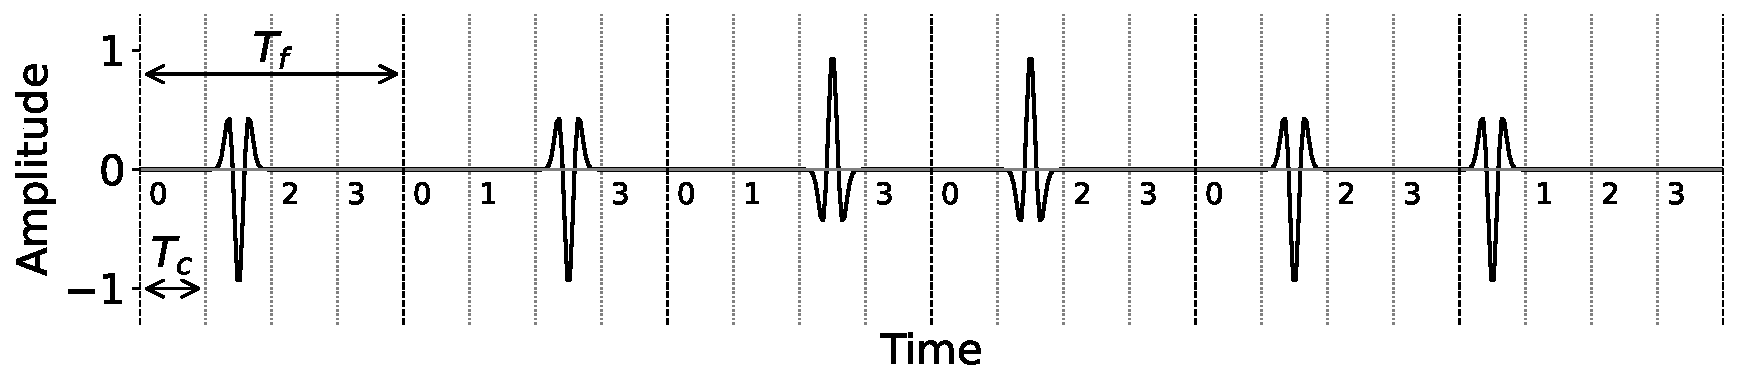
\includegraphics[width=0.9\textwidth]{Figures/theoretical_background/uwb_bpsk.pdf}
\centering
\caption{Conceptual illustration of the UWB BPSK modulation scheme.}
\label{fig:uwb-mod}
\end{figure}

Conversely, IR-UWB employs a fundamentally different approach by using a pulse-based modulation scheme that does not rely on a continuous wave carrier. To transmit the data, it typically uses ternary modulation, achieved through the combination of Burst Position Modulation (BPM) and BPSK:

\begin{itemize}
\item In BPM, the information is encoded by the temporal position of a pulse within the UWB symbol of duration $T_{\text{dsym}}$. The transmitted signal is given by:
\begin{equation}
S(t) = A p\left(t - b_n T_{\text{BPM}}\right),
\end{equation}
where $A$ is the pulse amplitude, $p(t)$ is the pulse shape, and $b_n \in \{0, 1\}$ is the modulating bit, selecting one of two available BPM intervals $T_{\text{BPM}} = T_{\text{dsym}}/{2}$.

\item In BPSK, the information is encoded by inverting the polarity of the transmitted pulse. The transmitted signal can be expressed as:
\begin{equation}
S(t) = A (1 - 2b_n) \, p(t),
\end{equation}
where $b_n \in \{0, 1\}$ is the modulating BPSK bit that determines the pulse phase.
\end{itemize}

\autoref{fig:uwb-mod} illustrates the concept of UWB BPSK modulation scheme~\cite{Sahinoglu2008UWB}. Here, each symbol, representing one bit, consists of a sequence of two impulses, transmitted in consecutive frames of duration $T_f$. The position of each pulse within its frame is defined by a time-hopping code $m \in \{0, 1, 2, 3\}$, used to minimize multi-user interference by pseudo-randomly selecting one of $M = 4$ slots of duration $T_c$. The polarity is modulated using BPSK to encode the data. The example on the figure effectively represents the binary sequence:
$$
\boxed{1\ 0\ 1}
$$ 
with time-hopping code: 
$$
\{1, 2\},\ \{2, 1\},\ \{1, 0\}.
$$

\paragraph{Bandwidth.}
The use of ultrashort pulses in UWB systems enables exceptionally high temporal resolution, which is critical for precise estimation of the signal's time of arrival and, consequently, accurate time-of-flight measurements. This capability is governed by the time-bandwidth uncertainty principle, which imposes a lower bound on the product of time duration $\Delta t$ and bandwidth $\Delta f$ of the signal:
\begin{equation} 
\Delta t \cdot \Delta f \geq \frac{1}{2}. 
\end{equation}
The spatial resolution $\Delta D$ associated with ToF-based ranging is therefore:
\begin{equation} 
\Delta D \geq \frac{c}{2\Delta f}, 
\end{equation}
where $c$ is the speed of light. Accordingly, larger bandwidths directly improve ranging precision.

In practical terms, achieving finer resolution in the time domain requires broader occupancy in the frequency domain. This time-frequency duality is formally described by the Fourier transform:
\begin{equation} 
\mathcal{F}{x(t)} = X(f) = \int_{-\infty}^{\infty} x(t) e^{-j2\pi ft} dt, 
\end{equation}
which decomposes a time-domain signal $x(t)$ into its frequency-domain representation $X(f)$. A canonical example is the Dirac delta function $\delta(t)$, which satisfies:
\begin{equation} \mathcal{F}{\delta(t)} = 1, \end{equation}
indicating that a theoretically infinitesimal pulse contains all frequencies with equal amplitude -- i.e., infinite bandwidth. While physical systems cannot generate true delta functions, UWB pulses (e.g., Gaussian monocycles or higher-order derivatives) approximate this behavior.

UWB's bandwidth of~\SI{500}{\mega\hertz} or more correlates with sub-nanosecond temporal resolution and centimeter-level ranging accuracy. In contrast, conventional narrowband systems (e.g., BLE, Wi-Fi) transmit signals with limited bandwidth (1–20~\si{\mega\hertz}), yielding a time resolution of tens to hundreds of nanoseconds. This restricts their temporal resolution, leading to ranging errors in the order of meters. Additionally, the usage of continuous waves makes them susceptible to multipath interference. Together, this renders narrowband technologies unsuitable for fine-grained localization in multipath-dense environments.

However, to estimate the ToF precisely, UWB still has to distinguish the actual direct signal path from multipath components. For this purpose, UWB relies on Leading Edge Detection (LDE) algorithms, which operate on CIR.

\section{UWB principles}\label{principles}
\subsection{UWB frame}

\begin{figure}[tbh]
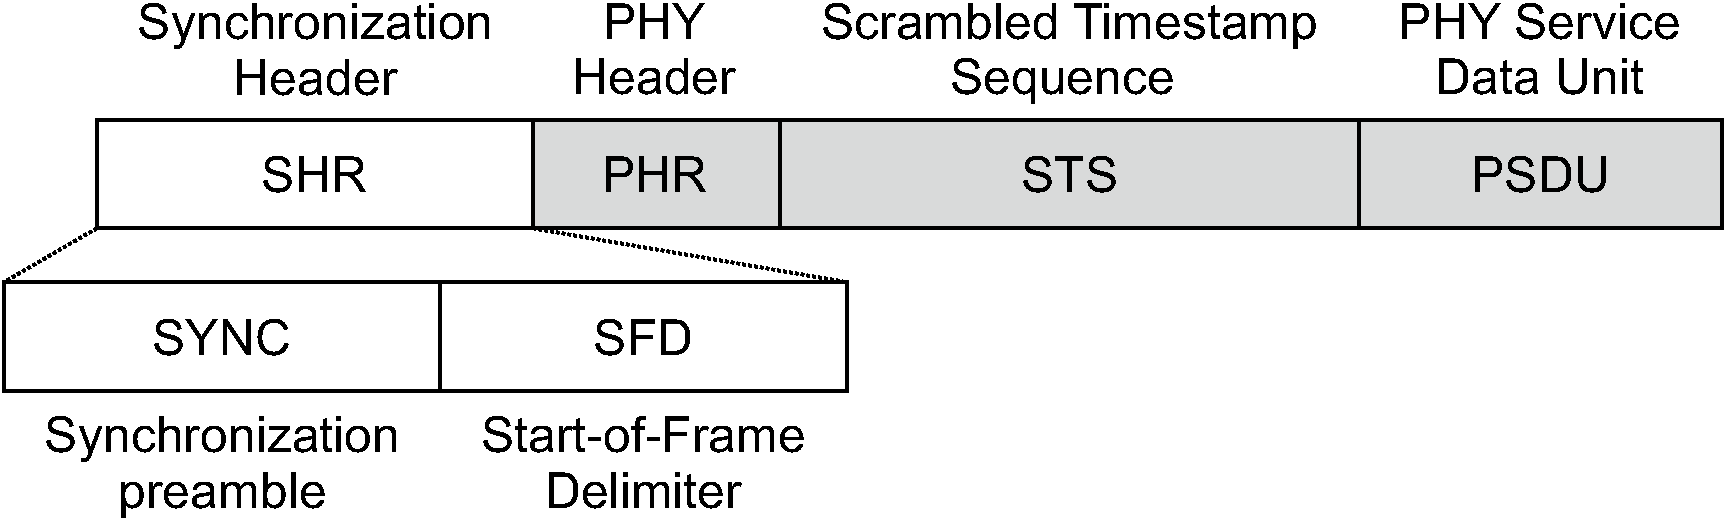
\includegraphics[width=0.75\textwidth]{Figures/theoretical_background/uwb_phy.pdf}
\centering
\caption{IEEE 802.15.4z UWB PHY frame structure. Gray fields are optional.}
\label{fig:phy}
\end{figure}

IEEE 802.15.4z-compliant UWB physical layer (PHY) frame format (\autoref{fig:phy}) follows the below structure:

\begin{itemize} 
    \item Synchronization Header (SHR): contains the preamble (SYNC) and Start-of-Frame delimiter (SFD) sequences, used for synchronization and time-stamping. 
    \item Physical Layer Header (PHR): encodes frame control information \emph{(optional)}. 
    \item Scrambled Timestamp Sequence (STS): provides additional security and precision timing support \emph{(optional; may also be positioned at the end of the frame)}. 
    \item PHY Service Data Unit (PSDU): PHY payload. Contains the transmitted information \emph{(optional)}. 
\end{itemize}

The synchronization header of the frame is particularly relevant for UWB ranging capabilities, as it contains the preamble used for CIR reconstruction. In SHR, a SYNC sequence, or preamble, is transmitted first. It consists of the repetition of known sequence codes. The codes used in the preamble are defined in the standard and are part of the family of codes known as perfect ternary sequences~\cite{mcelroy2014comparison}. These codes are constructed using a ternary alphabet $\{0, -1, 1\}$ to exhibit unique perfect periodic autocorrelation properties. 

The autocorrelation function of a sequence $\bm s$ of length $N$ for shift $\tau$ is given by:
\begin{equation}
R(\tau) = \sum_{i=0}^{N-1} \bm s_i \cdot \bm s_{(i+\tau) \bmod N}.
\end{equation}
A sequence has perfect periodic autocorrelation if all off-peak autocorrelation values are zero~\cite{blake2014construction}:
\begin{equation}
R(\tau) =
\begin{cases}
    N, & \tau \equiv 0\ (\bmod\, N),\\
    0, & \tau \not\equiv 0\ (\bmod\, N).
\end{cases}
\end{equation}
The perfect autocorrelation property ensures that once the presence of a transmission is detected by the receiver device, the remainder of the preamble can be used for CIR estimation~\cite{mcelroy2014comparison}.

\subsection{Channel impulse response}\label{cir_theory}

\begin{figure}[tbh]
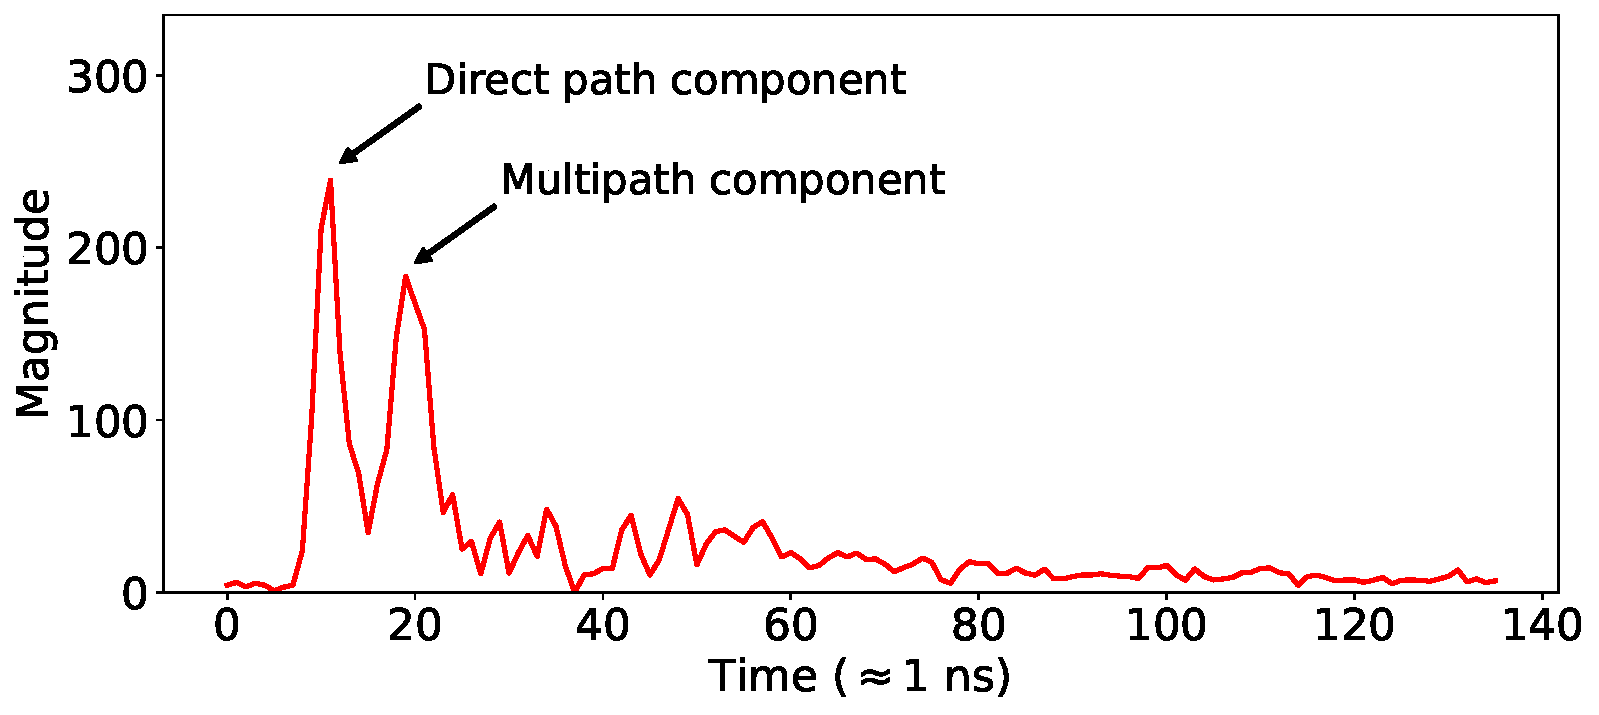
\includegraphics[width=0.75\textwidth]{Figures/theoretical_background/cir_sample.pdf}
\centering
\caption{Typical example of a measured channel impulse response.}
\label{fig:cir}
\end{figure}

CIR is the fundamental characteristic of any UWB system. The receiving device estimates CIR by correlating a known preamble sequence with a received signal. CIR $h(t)$ is often modeled as~\cite{cheraghinia2024comprehensive}:
\begin{equation}
h(t) = \sum_{i} a_i \delta(t - \tau_i) + \nu(t),
\end{equation}
where $a_i$ and $\tau_i$ represent the amplitude and delay of the $i$-th multipath component, respectively, $\delta(t)$ denotes the Dirac delta function, and $\nu(t)$ represents diffuse multipath components. The first term encapsulates multipath propagation phenomena, where the transmitted signal is propagated to the receiver through multiple paths, arriving with different delays. The second term models random noise, typically with additive white Gaussian noise (AWGN).

To this end, CIR characterizes how an impulse signal propagates through the wireless channel and captures the features of the propagation environment. A typical CIR accumulator is presented in \autoref{fig:cir}. The sampling interval of the CIR is equal to half of the period of the fundamental frequency (FF), which is typically around \SI{1}{\nano\second} for \SI{500}{\mega\hertz} FF. Consequently, each sample of the CIR corresponds to a distance of \SI{\approx 30}{\centi\metre} (given that the UWB signal propagates through the air medium). As was noted before, such high temporal resolution allows UWB to distinguish between multiple paths, achieving precise ToF estimation. This process is performed by the LDE algorithm.

\subsubsection{Leading edge detection}\label{lde}
\begin{figure}[tbh]
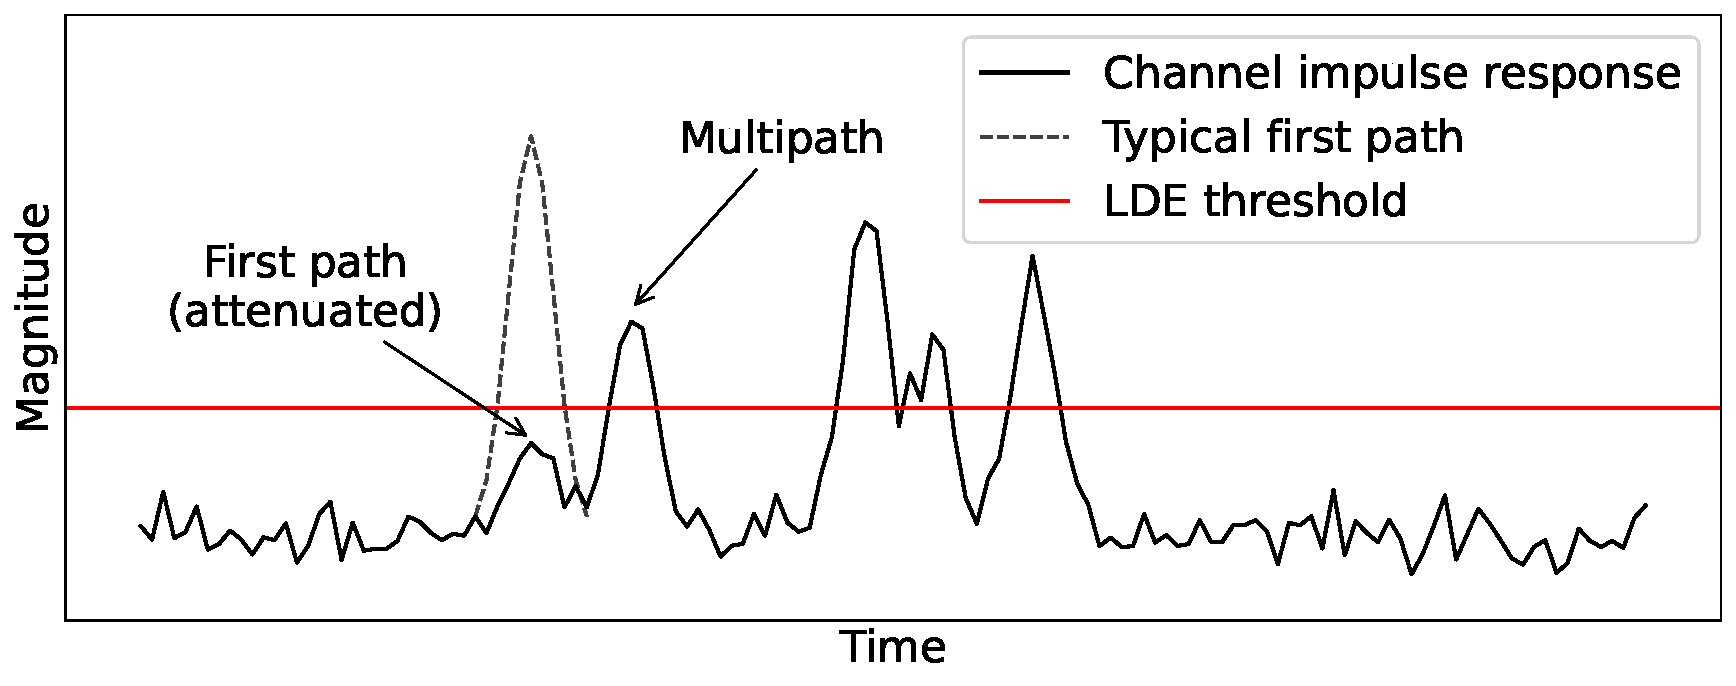
\includegraphics[width=0.8\textwidth]{Figures/theoretical_background/uwb_lde_error.pdf}
\centering
\caption{Conceptual illustration of undetected first path in the LDE process.}
\label{fig:lde-nlos}
\end{figure}
The LDE algorithm analyzes the CIR to determine the first path (FP) -- the earliest signal component corresponding to the time of arrival. In practical terms, LDE aims to distinguish the genuine FP from subsequent multipath components and background channel noise. This is accomplished by applying a threshold $\theta_{\text{LDE}}$, typically derived from the estimated noise floor:
\begin{equation}
\tau_{\text{LE}} = \arg \min_{\tau} \{ h(\tau) \geq \theta_{\text{LDE}} \},
\end{equation}
where $\tau_{\text{LE}}$ is the estimated arrival time of the first path.

Clearly, accurate identification of the FP is critical for precise ranging. Under LoS conditions, the LDE algorithm typically produces reliable timestamps. However, in severe NLoS cases, the direct path component may be attenuated to such an extent that it becomes effectively undetectable. As a result, the LDE algorithm may misidentify a reflected multipath component as the FP, leading to inaccurate time-stamping and, consequently, ranging error. This scenario is illustrated in \autoref{fig:lde-nlos}.

\subsection{Ranging techniques}
\subsubsection{Two-way ranging}\label{theory:twr}

\begin{figure}[tbh]
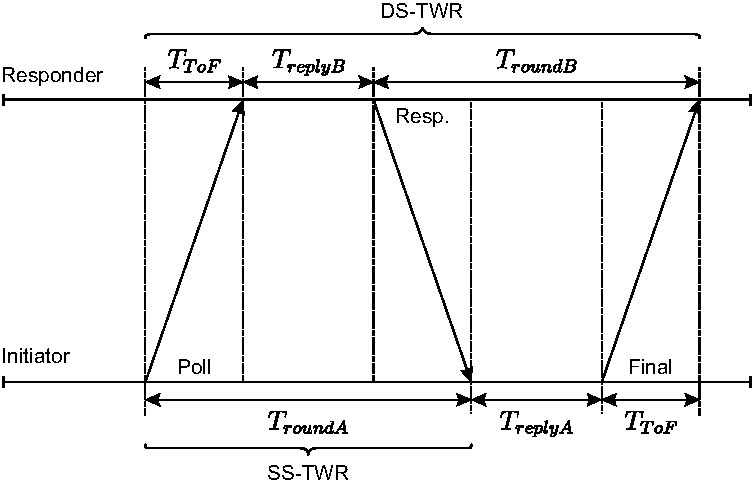
\includegraphics[width=0.75\textwidth]{Figures/theoretical_background/twr.pdf}
\centering
\caption[Two-way ranging exchange.]{Two-way ranging exchange (single-sided and double-sided).}
\label{fig:twr}
\end{figure}

ToF estimation with single, one-way communication requires precise clock synchronization between tag and anchor devices. This is extremely hard to achieve, as centimeter-level precision in ToF estimation requires the clock difference to be in the order of picoseconds. Therefore, UWB systems often rely on TWR to determine distance, eliminating the requirement for precise time synchronization between devices. TWR works by measuring the round-trip time of signals.

\paragraph{SS-TWR.}
The simplest form of TWR is single-sided TWR (SS-TWR), where a responder device (B) sends a \emph{Response} message upon receiving a \emph{Poll} request from the initiator device (A). \autoref{fig:twr} illustrates the ranging exchange in the TWR process. The ToF is then inferred from the following equation:
\begin{equation}\label{tof-ss}
T_{ToF} = \frac{1}{2} (T_{roundA} - T_{replyB}),
\end{equation}
where $T_{roundA}$ is the round-trip time, $T_{replyB}$ is the time delay at the responder, and $T_{ToF}$ is the time-of-flight. Under ideal conditions, $T_{ToF}$ can be precisely estimated. However, this estimate can still be largely affected by the clock drift~\cite{neirynck2016alternative}.

\paragraph{DS-TWR.} 
To mitigate clock drift errors, double-sided TWR (DS-TWR) adds a symmetrical exchange to SS-TWR by sending an additional \emph{Final} message from the initiator back to the responder upon receiving the \emph{Response}. Similarly to SS-TWR (\autoref{tof-ss}), in DS-TWR, the ToF is derived as follows: 
\begin{equation}
\begin{cases}
T_{roundA} = T_{replyB} + 2T_{ToF},\\
T_{roundB} = T_{replyA} + 2T_{ToF};
\end{cases}
\end{equation}
\begin{equation}
T_{ToF} = \frac{1}{4} (T_{roundA} - T_{replyB} + T_{roundB} - T_{replyA}).
\end{equation}

However, this approach still has a limitation due to the assumption that the reply delays $T_{replyX}$ will be equal on both sides~\cite{neirynck2016alternative}. 

\paragraph{ADS-TWR.}\label{adstwr}
A variation known as Alternative DS-TWR (ADS-TWR) has been proposed by Dries Neirynck et al.~\cite{neirynck2016alternative}. ADS-TWR eliminates the requirement for equal reply delays, reducing the complexity of the system and improving ToF estimation accuracy. Instead of relying on reply delay symmetry, it applies:
\begin{equation}
T_{ToF} = \frac{T_{roundA}T_{roundB} - T_{replyA}T_{replyB}}{T_{roundA} + T_{replyA} + T_{roundB} + T_{replyB}}.
\end{equation}

This method minimizes the impact of the clock drift error, making it more robust for practical implementations.

\subsubsection{Time-division multiple access}\label{tdma}

Generally, it is desirable to obtain the measurement result on the tag device to minimize system complexity. However, achieving this within the framework of DS-TWR necessitates that the measurement process be initiated by the anchor, as it would otherwise be necessary to introduce additional exchanges that would degrade the system's performance in terms of ranging frequency. Consequently, this introduces a requirement of synchronization  among multiple anchor devices to prevent simultaneous ranging attempts and avoid cross-interference.

Addressing this requirement typically involves the application of Time-Division Multiple Access (TDMA)~\cite{falconer1995time, Yanjun2021TDMA}, a channel access method that enables multiple devices to share the same communication channel by allocating distinct time slots for their respective ranging operations, thereby preventing signal collisions. The process is as follows:


\begin{itemize}
    \item the network controller (tag) assigns a time slot to each ranging device (anchor);
    \item devices are configured to transmit signals only within their allocated slots;
    \item receivers listen for and process incoming signals exclusively during the corresponding time slots assigned to each device, preventing overlap.
\end{itemize}

Originally, TDMA was used in satellite communication systems, but later, it was also adopted in UWB TWR-based systems.

\section{Sources of errors}\label{error_sources}

\begin{figure}[tbh]
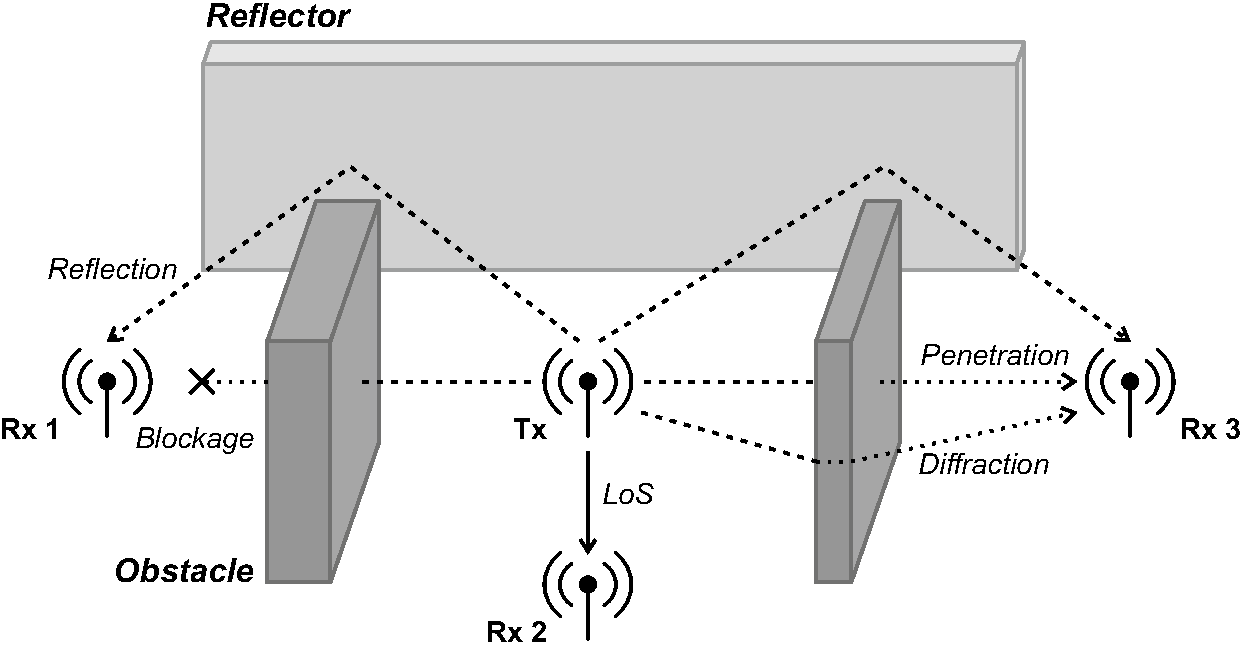
\includegraphics[width=0.8\textwidth]{Figures/theoretical_background/obstacles.pdf}
\centering
\caption[Illustration of error sources.]{Illustration of error sources. The transmitter (Tx) communicates with three receivers (Rx 1-3) under different conditions: complete direct signal blockage (Rx 1), LoS propagation (Rx 2), and multipath propagation (Rx 3) involving reflection, diffraction, and obstacle penetration.}
\label{fig:error_nlos}
\end{figure}

Despite the high precision of UWB-based ranging systems, several error sources affect their performance, particularly in indoor and multipath-rich environments. These include NLoS propagation, multipath interference, and refraction effects~\cite{dardari2009ranging}. The schematic in \autoref{fig:error_nlos} illustrates the principal NLoS conditions.

\paragraph{Multipath interference.}
Multipath occurs when multiple copies of the transmitted signal arrive at the receiver via different paths due to reflections, diffractions, and scattering. UWB systems are generally resilient to multipath because of their short pulses, which allow separation of distinct paths in the CIR. This phenomenon is discussed in \autoref{lde}. However, in dense multipath environments, the LDE algorithm can misclassify later multipath components as the actual direct path, introducing a positive bias in the estimated range:
\begin{equation}\label{multipath_err}
    \Delta d = \tau_i c,
\end{equation}
where $\tau_i$ is the delay of the $i$-th multipath component.

\paragraph{NLoS propagation.}
NLoS propagation occurs when the direct path between the transmitter and receiver is obstructed, and the first arriving signal is a reflected, refracted, or diffracted version of the original pulse. This also introduces a positive bias in the estimated range. In the case of partial NLoS, where the direct path still exists but passes through a refractive material (e.g., a wall or furniture), which slows the signal down, the measurement error is modeled as:
\begin{equation}
\Delta d = (\sqrt{\epsilon_r} - 1) d_o,
\end{equation}
where $d_o$ is the thickness of the obstacle, and $\epsilon_r$ is its relative permittivity.

In the case of complete blockage, the receiver can only observe the reflected or diffracted multipath signal components, therefore reporting the wrong distance estimate. This effect is illustrated in \autoref{lde}. The error model is analogous to the multipath case (\autoref{multipath_err}) described above. Empirically, the resulting range bias $b_r$ is often modeled as a log-normal random variable:
\begin{equation}
b_r \sim \text{Lognormal}(\mu, \sigma^2).
\end{equation}

This effect of error can be reduced by NLoS identification and mitigation techniques, such as machine learning models, discussed in \autoref{related_work}.

\paragraph{Geometric dilution of precision.}
In addition to measurement errors, the accuracy of UWB positioning systems is fundamentally influenced by the geometric configuration of anchor nodes.

This impact is quantified by the Geometric Dilution of Precision (GDOP), a metric that describes how uncertainty in distance measurements propagates to uncertainty in estimated position. Consider $N$ anchor nodes located at known positions $\mathbf{p}_{A_i} = (x_{A_i}, y_{A_i})$ for $i = 1, \dots, N$, and a tag at position $\mathbf{p}_T = (x_T, y_T)$. The measured distance from the tag to the $i$-th anchor is given by:
\begin{equation}
d_i = \|\mathbf{p}_T - \mathbf{p}_{A_i}\|.
\end{equation}

Linearizing the system of distance equations around an estimate $\mathbf{p}_0 = (x_0, y_0)$ yields the Jacobian matrix $H$, whose rows are unit direction vectors from the linearization point to each anchor:
\begin{equation}
H = \begin{bmatrix}
\frac{x_0 - x_{A_1}}{d_1} & \frac{y_0 - y_{A_1}}{d_1} \\
\vdots & \vdots \\
\frac{x_0 - x_{A_N}}{d_N} & \frac{y_0 - y_{A_N}}{d_N}
\end{bmatrix}.
\end{equation}
The GDOP is then defined as~\cite{Wang2022GDOP}:
\begin{equation}
\text{GDOP} = \sqrt{\text{trace}\left((H^\top H)^{-1}\right)}.
\end{equation}

Lower GDOP values correspond to better geometric configurations. The minimal GDOP in 2-D localization is theoretically attained when the target lies inside the convex hull formed by anchors placed at the vertices of a regular $N$-sided polygon, where $N$ is the number of anchors~\cite{Wang2022GDOP,Levanon2000GDOP}. Optimal anchor deployment is essential for reducing position uncertainty, especially in environments with unavoidable NLoS and multipath conditions.